\documentclass[tikz,border=5mm]{standalone}
\usepackage{amsmath, amssymb}
\usetikzlibrary{arrows.meta, backgrounds, fit, positioning}

% Custom styles for consistency
\tikzset{
    node style/.style={
        draw=black,
        fill=white,
        minimum width=1.8cm,
        font=\small,
        align=center,
        inner sep=4pt,
        outer sep=2pt,
    },
    solid arrow/.style={
        ->,
        >=Stealth,
        thick,
        shorten >=2pt,
        shorten <=2pt,
    },
    dashed arrow/.style={
        ->,
        >=Stealth,
        dashed,
        thick,
        shorten >=2pt,
        shorten <=2pt,
    },
    highlight region/.style={
        fill=gray!20,
        rounded corners=8pt,
        opacity=0.8,
    },
}

\begin{document}
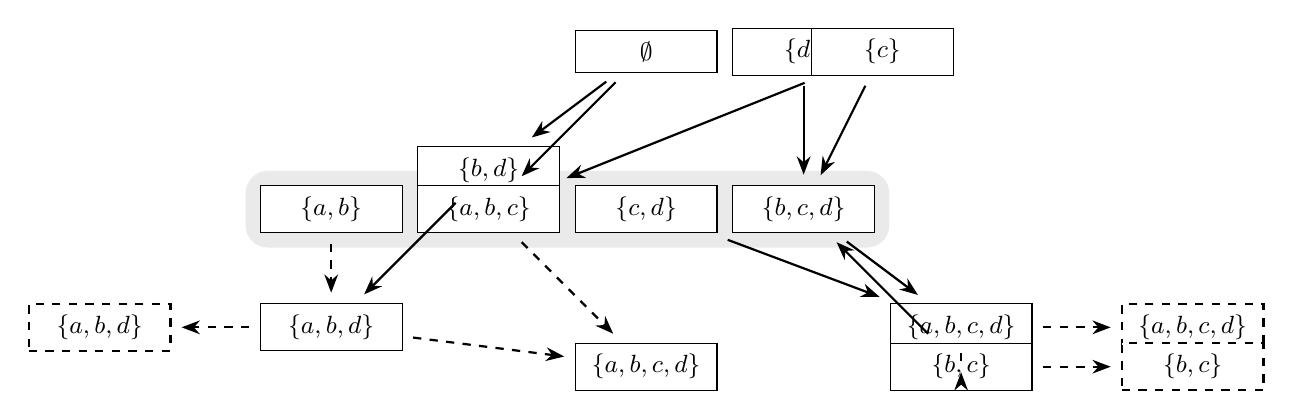
\begin{tikzpicture}[
    node distance=2.2cm and 2.5cm,
    >=Stealth, % Global arrow tip setting
]

% Define nodes
\node[node style] (empty) at (4,4) {$\emptyset$};
\node[node style] (d) at (6,4) {$\{d\}$};
\node[node style] (c) at (7,4) {$\{c\}$};

\node[node style] (bd) at (2,2.5) {$\{b,d\}$};
\node[node style] (ab) at (0,2) {$\{a,b\}$};
\node[node style] (abc) at (2,2) {$\{a,b,c\}$};
\node[node style] (cd) at (4,2) {$\{c,d\}$};
\node[node style] (bcd) at (6,2) {$\{b,c,d\}$};

\node[node style] (abd) at (0,0.5) {$\{a,b,d\}$};
\node[node style] (abcd) at (8,0.5) {$\{a,b,c,d\}$};

\node[node style] (abcd2) at (4,0) {$\{a,b,c,d\}$};
\node[node style] (bc) at (8,0) {$\{b,c\}$};

% Draw solid arrows
\draw[solid arrow] (empty) -- (bd);
\draw[solid arrow] (empty) -- (abc);
\draw[solid arrow] (d) -- (bcd);
\draw[solid arrow] (c) -- (abc);
\draw[solid arrow] (c) -- (bcd);
\draw[solid arrow] (bd) -- (abd);
\draw[solid arrow] (cd) -- (abcd);
\draw[solid arrow] (bc) -- (bcd);
\draw[solid arrow] (bcd) -- (abcd);

% Draw dashed arrows
\draw[dashed arrow] (ab) -- (abd);
\draw[dashed arrow] (abc) -- (abcd2);
\draw[dashed arrow] (bc) -- (bc);
\draw[dashed arrow] (abd) -- (abcd2);

% Highlight region
\begin{scope}[on background layer]
    \node[highlight region, fit=(ab)(bcd)] {};
\end{scope}

% Add additional dashed arrows for the external nodes
\draw[dashed arrow] (abd.west) -- ++(-1,0) node[left, node style] {$\{a,b,d\}$};
\draw[dashed arrow] (abcd.east) -- ++(1,0) node[right, node style] {$\{a,b,c,d\}$};
\draw[dashed arrow] (bc.east) -- ++(1,0) node[right, node style] {$\{b,c\}$};

\end{tikzpicture}
\end{document}